\section{Electrostatic discharges in the automotive field}
\subsection{General concept}
Electro-Static Discharges (ESD) are the result of the accumulation of electrostatic potential,
followed by a sudden discharge.

Tribo-electricity ? Charging mechanism or discharge mechanism ?

ESD usually involve current levels up to dozens of amps and thousands of volts, but with a time span of a few hundred nanoseconds.
The overall energy remains small, but the transient behavior is itself very harmful for electronic systems and integrated circuits.

\subsection{Generation mechanism in the automotive field}
The automotive field is generally considered a quite harsh environment for electronic devices.
This is also true in terms of ESD, due to two different mechanisms that continuously generate electro-static potential inside a vehicle.

When the car is moving on the road, the friction between the wheels and the road strips charges off-other, leading to the accumulation of
charges on the vehicle.

In a same approach, the friction between the car's body and the air mass also generates charge accumulation on the vehicle.

When the vehicle reaches critical electro-static potentials, a discharge will happen. Before reaching ground, the discharge will propagate through
the car's wires, body, and most importantly, electronic equipment.

Since the charging mechanism happens constantly during the car's operation, it is clear that electronic devices inside the vehicle will be regularly
exposed to ESD.

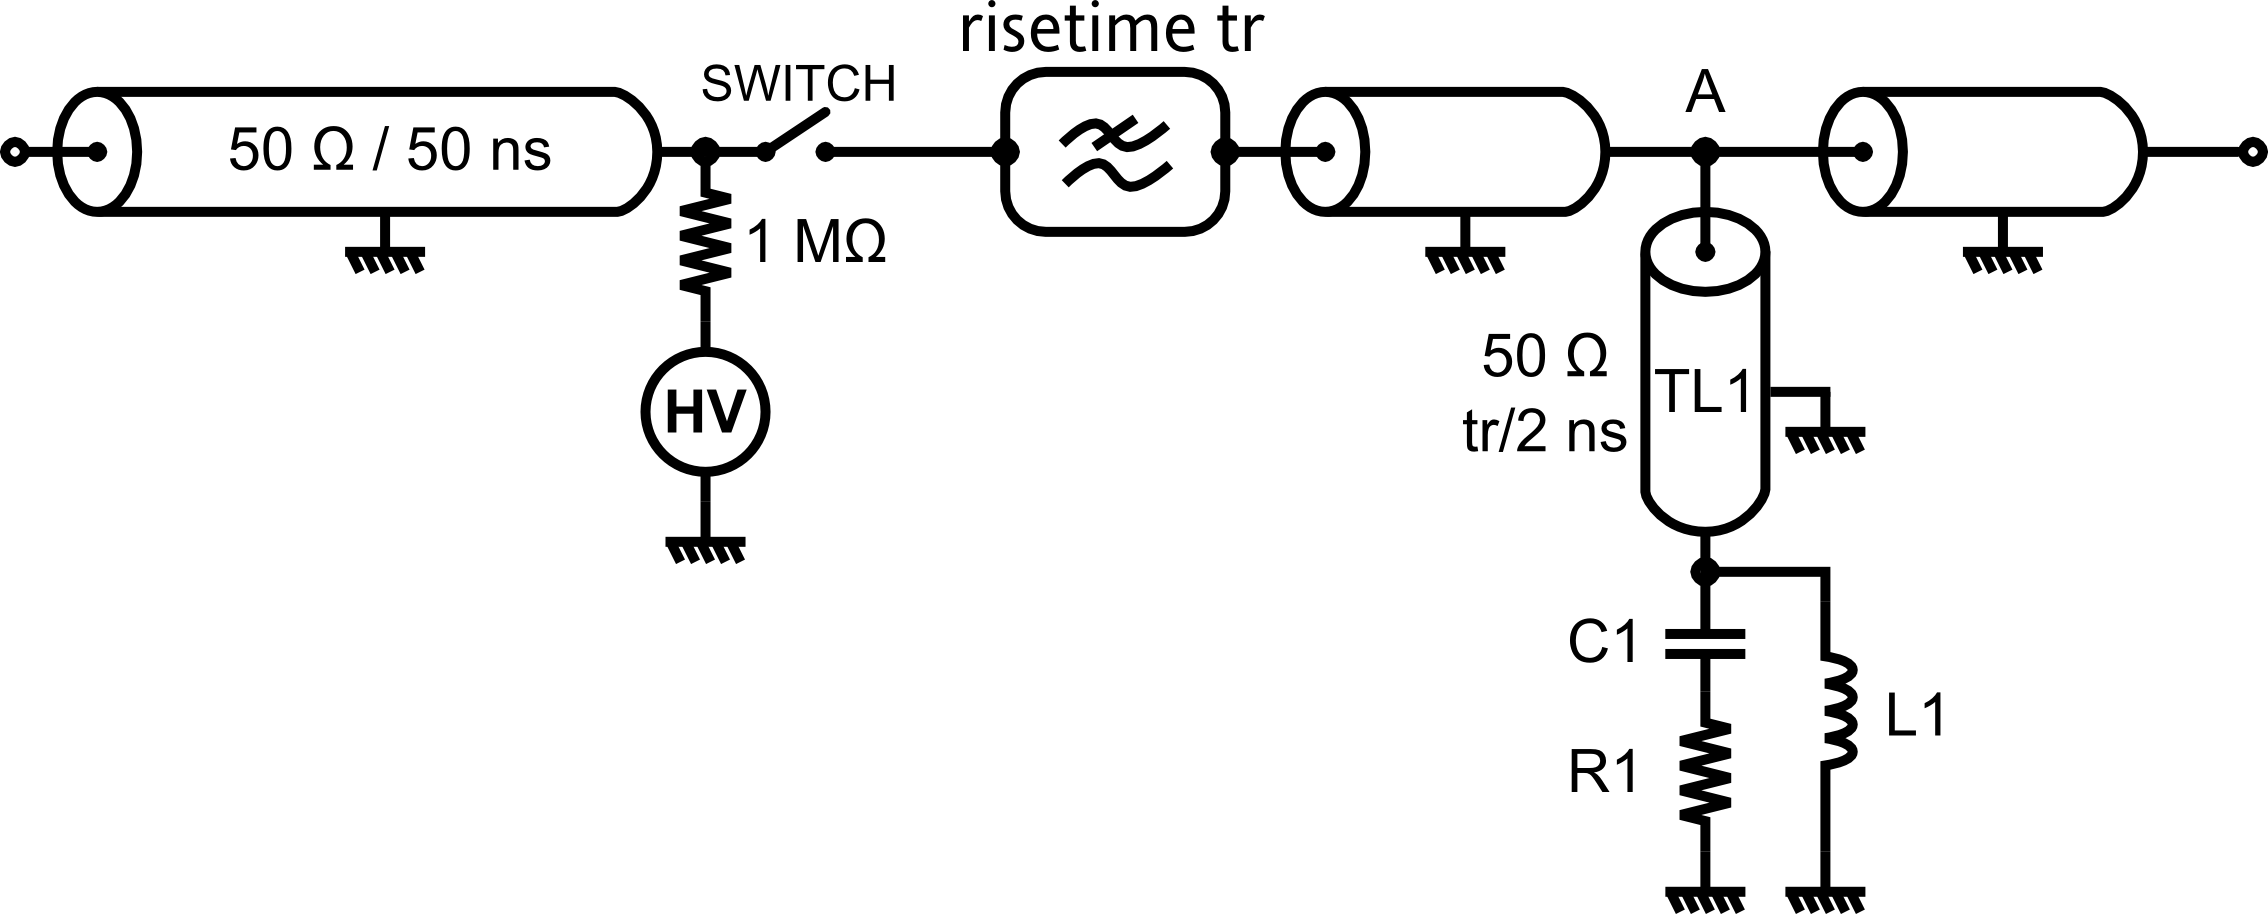
\includegraphics[width=\textwidth,height=\textheight,keepaspectratio]{src/1/figures/tlp_iec.png}
